\documentclass[11pt]{article}

\oddsidemargin0cm
\topmargin-2cm     %I recommend adding these three lines to increase the 
\textwidth16.5cm   %amount of usable space on the page (and save trees)
\textheight23.5cm  

\newcommand{\question}[2] {\vspace{.25in} \fbox{#1} #2 \vspace{.10in}}
\renewcommand{\part}[1] {\vspace{.10in} {\bf (#1)}}

\usepackage{graphicx}
\usepackage{amssymb,amsmath}

\begin{document}

\medskip                        % Skip a "medium" amount of space
                                % (latex determines what medium is)
                                % Also try: \bigskip, \littleskip


\begin{center}                  % Center the following lines
  {\Large Introduction to the Theory of Computation \\ Homework \#2} \\
  Brian Gianforcaro \\
  \date \\
\end{center}

\ttfamily

\question{1}{Proof: By structural induction}
\begin{center}
  \begin{itemize}
    \item Observe $({\epsilon}^{\mathcal{R}})^{\mathcal{R}} = ({\epsilon})^{\mathcal{R}} = {\epsilon}$
    \item Assume $ax^{\mathcal{R}} = x^{\mathcal{R}}a$
    \item Suppose $x = a`y$

    $((a'y)^{\mathcal{R}})^{\mathcal{R}} = ((a (ya'))^{\mathcal{R}})^{\mathcal{R}} $

    $ = (((ay)a'))^{\mathcal{R}})^{\mathcal{R}} $

    $ = (a'(ay)^{\mathcal{R}})^{\mathcal{R}} $

    $ = ((a'y^{\mathcal{R}})a)^{\mathcal{R}} $

    $ = ((a'y^{\mathcal{R}})a)^{\mathcal{R}} $

    $ = (y^{\mathcal{R}}a')^{\mathcal{R}} $

    $ = (y^{\mathcal{R}}a')^{\mathcal{R}} $

    $ = (a'y^{\mathcal{R}}) $

    $ = (a'y^{\mathcal{R}}) $
    
    $ = a'y $

  \end{itemize}
\end{center}

\indent \indent $\Box$

\question{2}{Diagrams the DFAs recognizing the following languages. The alphabet is $\{0,1\}$}

\part{a} $\{w | w$ begins with a 1 and ends with a 0$\}$
\begin{figure}[h!]
  \begin{center}
    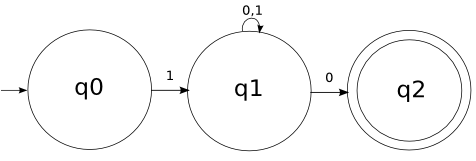
\includegraphics[scale=0.40]{2a.png}
  \end{center}
\end{figure}

\part{d} $\{w | w$ has length at least 3 and its third symbol is a 0$\}$
\begin{figure}[h!]
  \begin{center}
    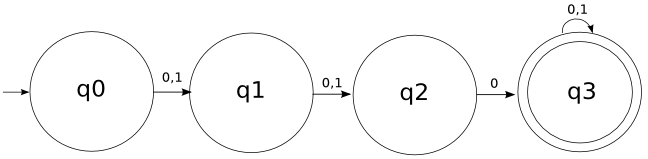
\includegraphics[scale=0.40]{2d.png}
  \end{center}
\end{figure}

\pagebreak

\part{i} $\{w | $every odd position of $w$ is a l$\}$  
\begin{figure}[h!]
  \begin{center}
    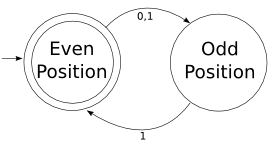
\includegraphics[scale=0.40]{2i.png}
  \end{center}
\end{figure}

\part{l} $\{w | w $contains an even number of Os, or contains exactly two 1s $\}$
\begin{figure}[h!]
  \begin{center}
    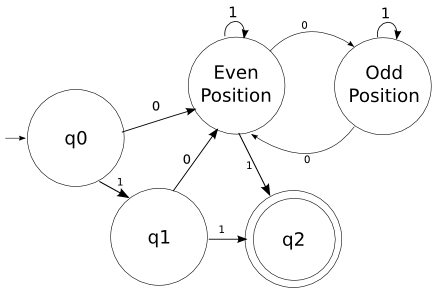
\includegraphics[scale=0.40]{2l.png}
  \end{center}
\end{figure}

\part{m} The empty set 
\begin{figure}[h!]
  \begin{center}
    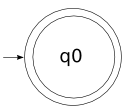
\includegraphics[scale=0.40]{2m.png}
  \end{center}
\end{figure}

\part{n} All strings except the empty string 
\begin{figure}[h!]
  \begin{center}
    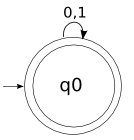
\includegraphics[scale=0.40]{2n.png}
  \end{center}
\end{figure}

\question{3}{}
\begin{figure}[h!]
  \begin{center}
    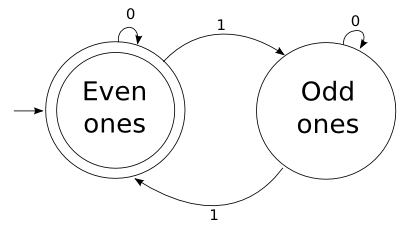
\includegraphics[scale=0.40]{3.png}
  \end{center}
\end{figure}


\question{4}{}
\part{a}
\begin{figure}[h!]
  \begin{center}
    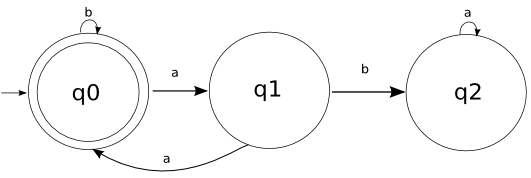
\includegraphics[scale=0.40]{4a.png}
  \end{center}
\end{figure}

\part{b}
  \begin{center}
  $Q_{k} = \{ q_{0}, q_{1}, q_{2} \} $

  ${\Sigma}_{k} = \{ a, b \} $

  ${\delta}_{k}(q_{0},a) = q_{1}$

  ${\delta}_{k}(q_{0},b) = q_{0}$

  ${\delta}_{k}(q_{1},a) = q_{0}$

  ${\delta}_{k}(q_{1},b) = q_{2}$

  ${\delta}_{k}(q_{2},a) = q_{2}$

  $F_{k} = \{ q_{0} \} $
  \end{center}
 
\question{6}{Exercise 1.7, Give NFAs with specified number of states}

\part{c}
\begin{figure}[h!]
  \begin{center}
    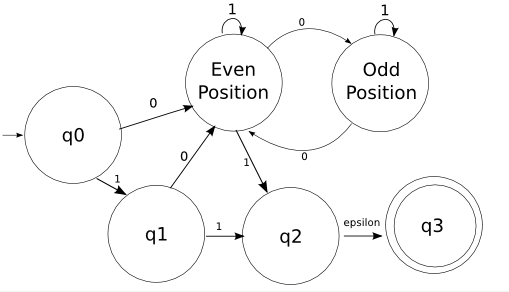
\includegraphics[scale=0.40]{6.png}
  \end{center}
\end{figure}

\question{7}{Calculate ${\delta}^{*}(q_{0}, 10)$.}
\begin{center}
  \begin{itemize}
    \item ${\delta}^{*}(q_{0}, 10) = \{q_{3}\}$
    \item ${\delta}^{*}(q_{3}, 10) = \{q_{6}\}$
    \item ${\delta}^{*}(q_{6},  0) = \{q_{5}\}$
    \item ${\delta}^{*}(q_{5},  {\epsilon}) = \{q_{3}\}$
    \item ${\delta}^{*}(q_{3},  {\epsilon}) = \{q_{2}\}$
  \end{itemize}
\end{center}


\question{8}{}

\part{a}

$\Sigma = \{0,1\}$

\begin{figure}[h!]
  \begin{center}
    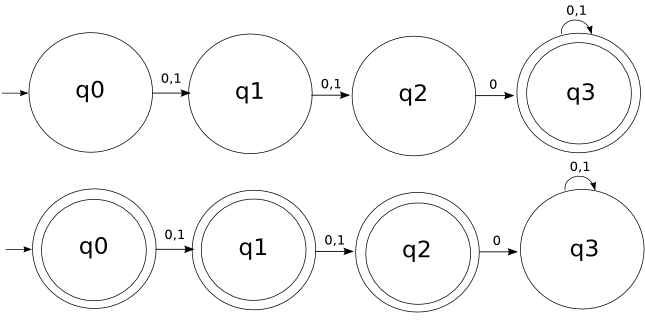
\includegraphics[scale=0.40]{8a.png}
  \end{center}
\end{figure}

\part{b}

$\Sigma = \{1,2,3\}$

\begin{figure}[h!]
  \begin{center}
    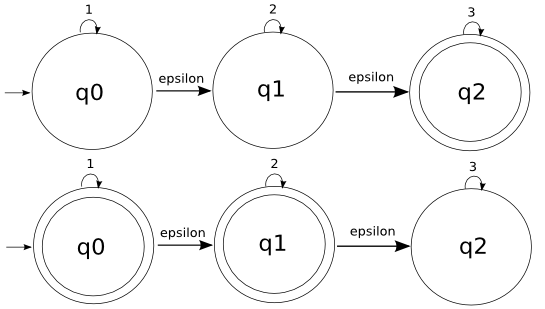
\includegraphics[scale=0.40]{8b.png}
  \end{center}
\end{figure}

Yes, the languages a NFA regonizes are closed under complement. 
The complement language will be recognized because of what we can do with epsilon transitions.

\pagebreak

\question{9}{Convert the following two NFA's to equivalent DFA's}

\part{a}

\begin{figure}[h!]
  \begin{center}
    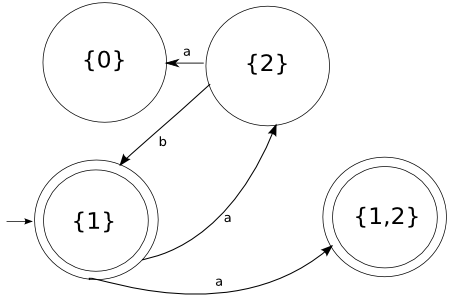
\includegraphics[scale=0.40]{16a.png}
  \end{center}
\end{figure}

\part{b}
\begin{figure}[h!]
  \begin{center}
    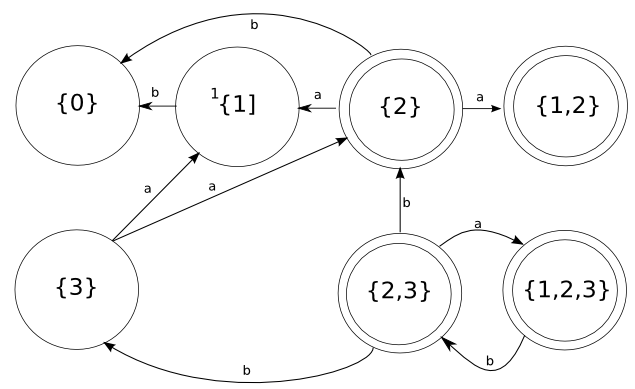
\includegraphics[scale=0.40]{16b.png}
  \end{center}
\end{figure}



\end{document}
